\documentclass{ecai}
\usepackage{times}
\usepackage{graphicx}
\usepackage{latexsym}
\usepackage{xspace}
\usepackage{hyperref}
\usepackage{amssymb}
\usepackage{algorithm}
\usepackage[noend]{algpseudocode}
\usepackage[numbers]{natbib}
\usepackage{notoccite}
\usepackage{framed}
\usepackage{amsmath}
\usepackage{tabularx}

\usepackage[dvipsnames]{xcolor}
\newcommand{\sergey}[1]{\textcolor{magenta}{{\sc Sergey:} #1}\xspace}
\newcommand{\samuel}[1]{\textcolor{green}{{\sc Samuel:} #1}\xspace}
\newcommand{\tias}[1]{\textcolor{blue}{{\sc Tias:} #1}\xspace}

\newcommand{\constraints}{\ensuremath{\mathcal{C}}\xspace}
\newcommand{\format}[1]{\textit{#1}\xspace}
\newcommand{\generategroups}{\format{generateAssignments}}
\newcommand{\extractgroups}{\format{extractGroups}}
\newcommand{\extracttables}{\format{extractTables}}
\newcommand{\learnconstraints}{\format{learnConstraints}}
\newcommand{\findassignment}{\format{findSolutions}}
\newcommand{\postprocess}{\format{pruneRedundant}}
\newcommand{\constrainttorder}{\format{orderedConstraints}}


\newcommand{\CName}{Name\xspace}
\newcommand{\CSignature}{Signature\xspace}
\newcommand{\CFunction}{Function\xspace}
\newcommand{\dependencies}{\ensuremath{\mathcal{D}}\xspace}
\newcommand{\groups}{\ensuremath{\mathcal{G}}\xspace}

\newcommand{\range}[3]{\ensuremath{#1[#2,#3]}}
\newcommand{\rangeto}[2]{#1{:}#2}
\newcommand{\rangeall}{:}

\newcommand{\eccalc}[2]{\ensuremath{#1 = #2}}
\newcommand{\ecrank}[2]{\eccalc{#1}{\mathit{RANK}(#2)}}
\newcommand{\ecfkey}[2]{\ensuremath{#1 \rightarrow #2}}
\newcommand{\ecalldiff}[1]{\ensuremath{\mathit{ALLDIFFERENT}(#1)}}
\newcommand{\eclookupf}[4]{\ensuremath{\mathit{LOOKUP}_{#4}(#1, #2, #3)}}
\newcommand{\eclookup}[4]{\eccalc{#1}{\eclookupf{#2}{#3}{#4}{}}}
\newcommand{\eclookupprod}[5]{\eccalc{#1}{#2 \times \eclookupf{#3}{#4}{#5}{}}}
\newcommand{\eclookupfuzzy}[4]{\eccalc{#1}{\eclookupf{#2}{#3}{#4}{fuzzy}}}
\newcommand{\ecperm}[1]{\ensuremath{\mathit{PERMUTATION}(#1)}}
\newcommand{\ecseries}[1]{\ensuremath{\mathit{SERIES}(#1)}}
\newcommand{\ecprod}[3]{\eccalc{#1}{#2 \times #3}}
\newcommand{\ectotal}[3]{\eccalc{#1}{\mathit{PREV}(#1) + #2 - #3}}
\newcommand{\ecproj}[2]{\eccalc{#1}{\mathit{PROJECT}(#2)}}
\newcommand{\ecaggc}[3]{\eccalc{#2}{\mathit{#1}(#3, col)}}
\newcommand{\ecaggr}[3]{\eccalc{#2}{\mathit{#1}(#3, row)}}
\newcommand{\ecsumc}[2]{\eccalc{#1}{\mathit{SUM}(#2, col)}}
\newcommand{\ecsumr}[2]{\eccalc{#1}{\mathit{SUM}(#2, row)}}
\newcommand{\ecaggif}[5]{\eccalc{#2}{\mathit{#1IF}(#3, #4, #5)}}
\newcommand{\ecsumif}[4]{\eccalc{#1}{\mathit{SUMIF}(#2, #3, #4)}}
\newcommand{\ecsumprod}[3]{\eccalc{#1}{\mathit{SUMPRODUCT}(#2, #3)}}

\newcommand{\luc}[1]{{\textcolor{red}{#1}}}





%%\ecaisubmission   % inserts page numbers. Use only for submission of paper.
                  % Do NOT use for camera-ready version of paper.

\begin{document}

\title{Tabular Constraint Learning}

\author{Name1 Surname1 \and Name2 Surname2 \and Name3 Surname3 \institute{KU Leuven, Belgium, email: firstname.lastname@kuleuven} }

\maketitle

\begin{abstract}
  abstract
\end{abstract}

\section{Introduction}
<<<<<<< HEAD
Millions of people across use spreadsheets everyday. Yet, many people lack a complete understanding of the structures and existing dependencies in the data. Indeed, the most useful part of spreadsheets is often the formulas and often these formula disappear, when a file is exported and shared as a CSV file. This brings us to the question: can we discover or reconstruct structural relations in flat tabular spreadsheet data? [in a general way that allows declarative specification of constraints to discover]

Let us have a look at the example in Figure \ref{fig:main_example}. Certainly there are several constraint present in the data and even the names in the headers already suggest the usage of standard spreadsheet operations such as \textit{average} or \textit{sum}. If we look at the Table 1 and at the first row in the Table 2, it is clear that one could have selected the column called \textbf{1st Quarter} in the Table  in the Table 11, clicked on the \textit{SUM} function and then just used the drag fill handle to apply the formula to the other columns. Similarly, that would work for the second (\textit{Average}), third (\textit{Min})  and forth (\textit{Max}) rows in Table 2. I.e., all operations are vectorized and make use of the standard spreadsheet operations. 

It is not hard to see that computation goes not only in columns but in rows as well: if we sum the values in Table 1 in the first row in all four quarters, we obtain the seventh column in Table 1. That gives us already a hint how this problem is different from the standard data mining setting, when the data is in rows and variables are in columns. Here everything is mixed, also some values are missing in the results, some missing the arguments, even a header might have missing values. The data is relational on the one hand, since we have multiple tables with relationships between them. And on the other hand, the data is numeric, since people tend to use spreadsheets for financial and accounting computations, which is heavily numeric.

This makes tabular data understanding and constraint learning new and challenging, and it is not only challenging for a machine but for a human as well. Due to the complexity of numeric computations in spreadsheets, people often fail to grasp the properties of the data, which leads to so called the \textit{Spreadsheet risk}\footnote{\url{https://en.wikipedia.org/wiki/Spreadsheet\#Spreadsheet_risk}} and even caused major flaws in the famous economics papers \cite{flaw_excel} and billion-losses in the financial industry \cite{spreadsheet_risk_loss}. Tabular constraint learning provides a potential cure by indicating learned constraint violations and suggesting possible fixes.
=======
Millions of people across the world use spreadsheets everyday.
Yet, many people lack a complete understanding of the structures and existing dependencies in the data.
Indeed, the most useful part of spreadsheets is often the formulas and often these formula disappear when a file is exported and shared, for example as a CSV file.
This brings us to the question: can we discover or reconstruct structural relations in flat tabular spreadsheet data?
Moreover, can we accomplish this task in a general way that allows declarative specification of constraints to discover?

\samuel{Maybe slightly more formal:}
Let us look at an example in Figure~\ref{fig:main_example}, the header names already suggest the usage of standard spreadsheet operations such as \textit{average} or \textit{sum}.
If we look at Table~1 and at the first row in Table~2, it is clear that one could have selected the column called \textbf{1st Quarter}, clicked on the \textit{SUM} function and then just used the drag fill handle to apply the formula to the other columns.
Similarly, that would work for the second (\textit{Average}), third (\textit{Min})  and forth (\textit{Max}) rows in Table 2.
I.e., all operations are vectorized and make use of the standard spreadsheet operations.

Examining Table~1 also shows that computations are not only performed column-wise but row-wise as well: the cells in the column \textbf{Total} are obtained by taking the row-wise sum of the previous four columns.
\samuel{Maybe slightly more formal:}
That gives us already a hint how this problem is different from the standard data mining settings, when the data is in rows and variables are in columns. Here everything is mixed, some values are missing in the results, some missing the arguments, even a header might have missing values. The data is relational on one hand, since we have multiple table with relationships between them. And on the other hand, the data is numeric, since people tend to use spreadsheets for financial and accounting computations, which is heavily numeric.

Given these novel aspects, we conclude that understanding and learning constraints in tabular data is a new and challenging problem setting.
Futhermore, it is not only challenging for a machine but for a human as well.
\samuel{Maybe slightly more formal:} Due to the complexity of numeric computations in spreadsheets, people often fail to grasp the properties of the data, which leads to so called the Spreadsheet risk\footnote{\url{https://en.wikipedia.org/wiki/Spreadsheet\#Spreadsheet_risk}} and even caused major flaw in the famous economics papers \cite{flaw_excel} and caused billion-losses in the financial industry. Tabular constraint learning provides a potential cure by indicating learned constraint violations and suggest possible fixes.
>>>>>>> fc6f339fbf88c9c55ff5168114106612d5c63c0c

\sergey{bullet points for Luc and Tias to rework introduction}\\
\textbf{Motivation}:
\samuel{Suggest better table layouts / formula translation}
\begin{itemize}
  \item File generated from model, model got lost, need to reconstruct
  \item Constraint programming is hard - is Excel hard?
  \item Avoid manual analysis, provide selection of constraints
  \item Error checking
  \item Completion, gain speed and insights (Complicated constraints, also complicated to verify, too much output)
\end{itemize}

\textbf{Novelty:}
\begin{itemize}
  \item Unsupervised setting (contrary to flashfill, etc)
  \item Numeric, different constraints (contrary to single textual function solution in flashfill, etc)
  \item Data format (2D) -- data is no longer in rows like a classic ML or DM settings
  \item Declarative, general / modular, stacking of constraint problems
\end{itemize}

\sergey{need to elaborate the example here: like in a story}

\begin{figure*}[tbh]
  \begin{center}
    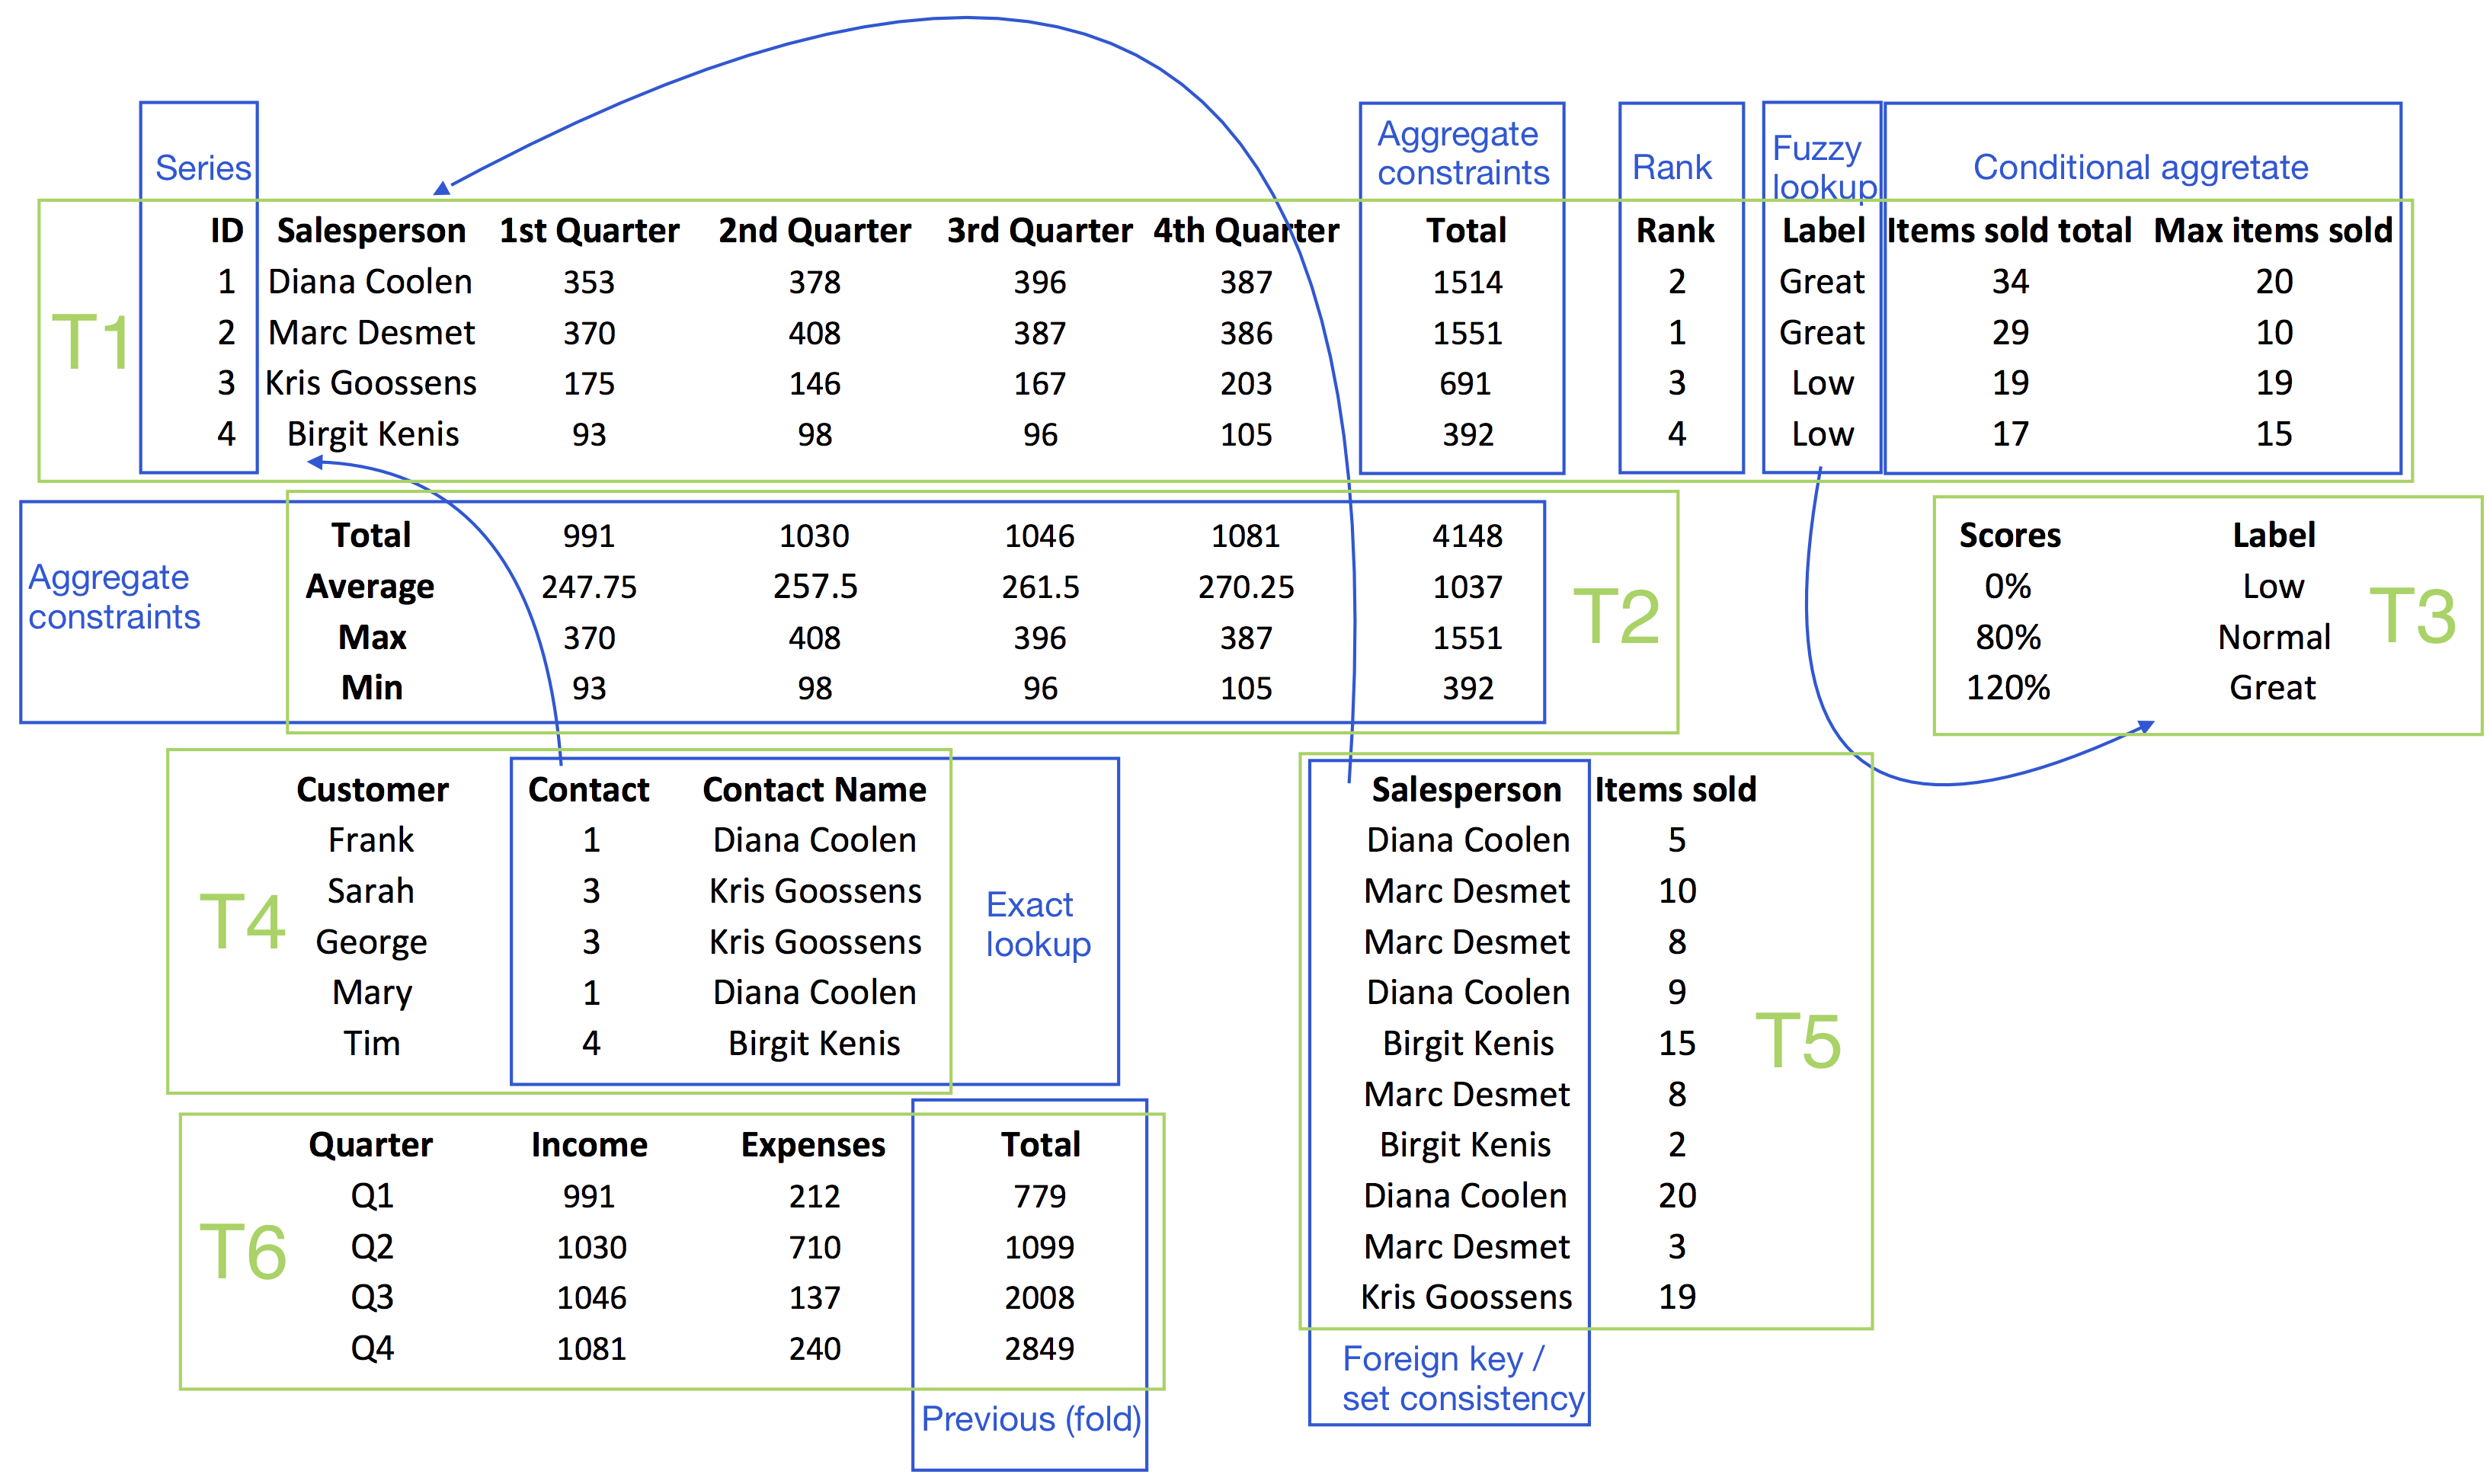
\includegraphics[width=0.75\textwidth]{figures/Demo.png}
  \end{center}
  \vspace{-10pt}
  \caption{An example of constraint reconstruction (in blue) with indicated groups (in green)}
  \label{fig:main_example}
\end{figure*}

\section{Formalization}
\samuel{Explain concepts on example}
\sergey{subgroup notation, rework the solution definition}
\subsection{Groups, Type-consistency and Constraints}
In this work we focus on spreadsheet data, which is physically one big table, but conceptually often consists of multiple tables, see Figure~\ref{fig:main_example} for an example.
Formally, a table is an $n \times m$ matrix, each table entry is called  a \textit{cell}.

Each cell has a {\em type} which can be numeric or textual.
The numeric type has two subtypes: integers and floats.
We also consider the special element called \textit{None}, which can be either type: numeric or textual.
A set of cells is called \textit{type-consistent} iff all cells in the set are either numeric or textual.
%Certain constraints, such as \textit{rank} or \textit{series}, make use of the numeric subtype by requiring its arguments to be integers.

We consider various sets of cells in tables:
\begin{itemize}
  \item {\bf Cells}: Each entry in the matrix/table is called  a \textit{cell}.
  We use the notation $T[a,b]$ to refer to a particular cell in the table~$T$ at the row with index~$a$ and the column with index~$b$.
  \item {\bf Columns and rows}: To refer to the $a$-th row (column) we use the following syntax $T[a,{:}]$ ($T[{:},a]$), to refer to a subrange from $a$ to $b$ we use $T[a{:}b,]$ ($T[,a{:}b]$).
  \item
  A \textit{vector} is either a column or a row that is type-consistent.
  If a vector is a row (column), we say that it has a \textit{row} (\textit{column}) orientation.
  \item
  A \textit{group} is a subrange of vectors with the same orientation in a table.
  We use the following notation to refer to a row (column) group $G$ in a table $T$ with rows (columns) ranging from $a$ to $b$: $G = T[a{:}b,:]$ ($G = T[{:},a{:}b]$), where $a,b$ are natural numbers.
  We denote as the \textit{length} of a row (column) group $G$, written as \textit{length(G)}, the number of its columns (rows). We call a group $G$ \textit{numeric} (\textit{textual}, etc), written as \textit{numeric(G)}, if \luc{all?????} its vectors contain numeric (textual, etc) elements.
  \item
 A \textit{subgroup} $g$ is a subrange of vectors belonging to a group $G$. If the subgroup $g$ must contain only one vector, we write $g \in G$.
%We refer to a subgroup of a group $G$ in \groups as $g$. A \textit{subgroup} $g$ is a subrange of vectors in a group $G$. If a subgroup $g$ must contain only one vector, we write $g \in G$.
% A \textit{subgroup} $G'$ is a subrange of vectors belonging to a group $G$. If the subgroup $\{v\}$ must contain only one vector, we write $v \in G$.
\end{itemize}
For notational convenience, we will refer to cells with $C$ \sergey{maybe better name? confusing with constaraints},  to vectors with $V$, and to groups and subgroups with $G$. 

When we do not want to distinguish between cells, columns, rows, vectors or groups, we shall talk about a {\em set of cells}.
\luc{add an example of group/ subgroup}



A \textit{Spreadsheet constraint} is a triple \textit{(\CName, \CSignature, \CFunction)}. Let us elaborate on each of them. 
\begin{itemize}
\item
\textit{\CName} is the textual name of the constraint together with the list of its variables $v_1,\dots,v_n$.
\item
  \textit{\CSignature} is a constraint specifying the properties of the group assignments, corresponding to the variables $v_1,\dots,v_n$ in \CName, such as their types, e.g., requiring them to be integers or constraining the sizes, e.g. the length of vectors in the arguments must be equal. These are constraints on the group meta-information not on the actual group content. 
\item \textit{\CFunction} is a constraint specifying that the data in the subgroups satisfies the function.

\paragraph{Example}
\sergey{need to use this below:}

  For example, a spreadsheet constraint \textit{rank} has \CName \textit{$v_y$ = RANK($v_x$)}, where $v_x$ and $v_y$ are the variables; its \CSignature is: the subgroup assigned to $v_x$ must be numeric, $v_y$ must be integer and the length of vectors in $v_x$ is the same as in $v_y$; its \CFunction is the following constraint: the mapping $\{ v_x \mapsto g_x, v_y \mapsto g_y \}$ is a solution iff $g_x \in G_x, g_y \in G_y$ ($G_x \in \groups, G_y \in \groups$) and each value in $g_x$ has the rank (possibly with ties) specified in $g_y$. 


The constraint \textit{rank} has
\begin{itemize}
\item \CName = \textit{$g_Y$ = RANK($g_X$)}, where $g_X$ and $g_Y$ are the group variables;
\item \CSignature = subgroup $g_X$ (associated with X) is numeric, $g_Y$ is integer and the length of vectors in $g_X$ is the same as in $g_Y$; and
\item
\CFunction = \textit{$g_Y$ = RANK($g_X$)} iff $g_X \in G_X, g_Y \in G_Y$ and each value in $g_X$ has the rank (possibly with ties) specified in $g_Y$.
\end{itemize}


We can now define a classical constraint satisfaction problem on tables.
A {\em constraint satisfaction problem} (CSP)  consists of 1) a set of cells, and 2) a set of constraints over those cells.
Notice that the constraints specify the types (or the domains) that one encounters in traditional CSPs.
Notice also, that as in traditional CSPs, the CSP problem defines the variables (the cells) of the problem
as well as the constraint that should hold amongst them. The task of CSP-solvers is then to find an assignment
to the variables that satisfies all the constraints. The distinction between variables (cells) and their assignments (their values)
is important here. So, when we speak about cells, vectors and groups, we refer to the variables;
when we talk about values, assignments or instances, we refer to the values these cells take in a particular "instantiated" table.

While the traditional CSP problem is given a set of cells and a set of constraints,
and the task is to find an assignment, the {\bf inverse CSP} or the {\bf Tabular Constraint Learning Problem}.
the can be defined as follows.\\
\\
{\bf Given }
\begin{itemize}
\item
a set of instantiated tables (so all cells have values) ${\cal T}$;
\item
a set of possible constraints ${\cal C}$;
\item
a set of possible groups for the tables ${\cal G}$;
\end{itemize}
\noindent
{\bf Find}  the set $C\subset {\cal C}$ that contains all constraints $c(G_1, ... , G_N)$ that 1) are satisfied  in ${\cal T}$, 2)
for which
all $G_i \in {\cal G}$ and  3)  $c(G_1, ... , G_N)$ satisfies the signature of the constraint $c$.


\luc{ADD/REFER TO EXAMPLE}

<<<<<<< HEAD


Let us now define what is a tabular solution for a spreadsheet constraint in general. Let $C$ denote a spreadsheet constraint, $S$ a mapping from variables to the subgroups of \groups, and $C^S$ the constraint $C$, in which all variables are substituted with the corresponding subgroups from $S$, then $S$ is a \textit{tabular solution} to $C$ iff both $\CSignature^S$ and $\CFunction^S$ hold.



\section{Problem Statement}
\sergey{should reflect all the changes, Luc wants to introduce constraint satisfaction into problem statement, maybe we should move the definition of a solution here? Like a solution is actually constraint satisfaction?}
In the previous section we introduced the problem of tabular constraint learning informally using the example in Figure \ref{fig:main_example}. Here we formalize the statement in terms of spreadsheet constraints and group assignments as follows: 
=======
%A \textit{tabular solution} $S$ to a spreadsheet constraint $C$ (with $n$ variables) is a subgroup assignment $(g_1, \dots, g_n)$ where $g_i$, such that $(g_1,\dots,g_n)$ satisfies both the \CSignature and \CFunction of the constraint $C$. \sergey{to finish this definition later, need to say that $g_i$ is the subgroup assigned to the $i$-th variable in $C$}

\section{Problem Statement}
\sergey{should reflect all the changes, Luc wants to introduce constraint satisfaction into problem statement, maybe we should move the definition of a solution here? Like a solution is actually constraint satisfaction?}
In the previous section we introduced the problem of tabular constraint learning informally using the example in Figure \ref{fig:main_example}. Here we formalize the statement in terms of spreadsheet constraints and group assignments as follows:
>>>>>>> fc6f339fbf88c9c55ff5168114106612d5c63c0c

\begin{minipage}[c]{14em}
  \vspace{5pt}
  \begin{tabular}{ll}
    \multicolumn{2}{l}{{\textbf{Tabular Constraint Learning Problem}}}\\
    \vspace{-4pt}
    &\\
    \textbf{Given:}& the set of all groups $\groups$ and of spreadsheet constraints $\constraints$\\
    \textbf{Find:}&  all tabular solution $S$ in \groups for each constraint $c$ in \constraints \\
  \end{tabular}
  \vspace{6pt}
\end{minipage}

  The key observation here is that essentially the problem is a constraint enumeration problem, where each constraint is independent. This property comes from fact that in spreadsheets each formula is applied based on the existing data in the cells. This allows learning constraints independently of each other by examining constraint satisfaction on the groups.


  In theory each constraint is independent and equally useful. In practice, however, things are different. Assume that for some $g_x$ both \textit{series($g_x$)} and \textit{alldifferent($g_x$)} hold. From a user's perspective the last solution is useless, since he or she already knows that the series constraint implies the alldifferent constraint. To capture this condensed representation \cite{condensed} of solutions, we have introduced a specificity (generality) order between constraints, which is depicted using solid (dashed) arrows in Figure \ref{fig:learning_order}. This matters from implementation perspective as well, if we discovered that $g_x$ is not a permutation, then $g_x$ should not be tested for the series constraint at all. A solid lines from $C_1$ to $C_2$ indicates that $C_2$ is \textit{more specific} than $C_1$ and if $S$ is not a solution to $C_1$, then it is not a solution to $C_2$. A dashed arrow from $C_1$ to $C_2$ indicates that $C_1$ is \textit{a more specific} constraint than $C_2$ and therefore if $S$ is a solution for $C_1$ it should not be tested for $C_2$.

We call a tabular solution $S$ to a constraint $C$ \textit{the most specific} wrt \dependencies, iff there is no other constraint $C'$ for which $S$ is a solution and $C'$ is more specific in \dependencies.


Let us introduce the version of tabular constraint learning that takes into account the specificity relation between constraints.

\begin{minipage}[c]{14em}
  \vspace{5pt}
  \begin{tabular}{ll}
    \multicolumn{2}{l}{{\textbf{Condensed Tabular Constraint Learning Problem}}}\\
    \vspace{-4pt}
    &\\
    \textbf{Given:}& the set of all groups $\groups$ and of spreadsheet constraints $\constraints$,\\
    & a constraint specificity DAG \dependencies \\
    \textbf{Find:}& all the most specific wrt \dependencies solutions $S$ in \groups\\
    & for each $c$ in \constraints \\
  \end{tabular}
  \vspace{6pt}
\end{minipage}

This version explicitly takes into account the specificity of the constraints and invalidates some of the solutions that are entailed by the tabular other solutions.

\section{Approach to Tabular Constraint Learning}
\sergey{Luc wants this to be more intuitive, should we just add some examples here to make it easier to follow and refer to the running example?}
As we have seen the statement before we assume the set of groups to be given. It is often, however, not the case and a possible approach is to extract the groups from the CSV file directly. In our system, we have implement the group construction step using the type-consistency check. \sergey{Samuel, we need details here, I think} In general, separating data from a header is a task on its own  \cite{header} and goes beyond the scope of this paper.

Another solution to the group extraction problem is to make it interactive, when a user can select the groups in the spreadsheet or correct automatically generated groups. We regard this approach to be a possible future direction in the system development. Later in the paper we assume the groups to be given.

Now we describe how the problem of Condensed Tabular Constraint Learning can be solved. The algorithm mimics the structure of the problem in the following way: first we need to order constraints in the order of specificity, then for each constraint we need to generate possible candidate groups, and in the next step we find the subgroups satisfying the constraint. After an iteration we accumulate all solutions and proceed to the next constraint.

\begin{algorithm}[thb]
  \begin{algorithmic}
    \footnotesize
    \State \textbf{Input:} $\groups$ -- groups, $\constraints$ -- Spreadsheet constraints, \dependencies -- dependency graph
    \State \textbf{Output:} $S$ -- learned constraints with their satisfaction assignments
    \State $S \gets \emptyset$ \Comment{The set of solutions}
  \For{$c \in \constrainttorder(\constraints,\dependencies)$}
  \State $v_1, ..., v_n =$ variables of $c$
    \For{$v_1{:}~G_1, \dots, v_n{:}~G_n \in \generategroups(c, G, S, \dependencies)$}
      \State $S \gets S \cup \findassignment(c, v_1{:}~G_1, \dots, v_n{:}~G_n, S, \dependencies)$
    \EndFor
  \EndFor\\
\Return $S$
\end{algorithmic}
\caption{Tabular constraint learning}
\label{algo:tcl}
\end{algorithm}
Essentially, our Algorithm \ref{algo:tcl} has three steps: constraint ordering, candidate group generation and subgroup satisfaction search, which is in line with the ``generate-and-test'' paradigm that is well-known in AI \cite{whaisasp}. Let us elaborate on each step in detail.

\samuel{Running example (RANK?)}

\subsection{Constraint ordering} $\constrainttorder(\constraints,\dependencies)$ uses the DAG \dependencies in Figure \ref{fig:learning_order} in the following way: all constraints are generated in the topological order of \dependencies.
Solid edges point from more general to more specific constraints.
Therefore, if there is a solid edge from $C_1$ to $C_2$, then a set of subgroups satisfying $C_2$ must contain the subgroups satisfying $C_1$.

Dashed edges represent the inverse relationship, pointing from specific to more general constraints.
If there is a dashed edge from $C_1$ to $C_2$, then a set of subgroups satisfying $C_2$ may not contain a subset that also satisfies $C_1$.

Thus, \dependencies describes a partial order in which constraints should be learned.
Some constraints have no dependencies (omitted from the figure) and can be learned independently.
Generally, a parallel version of the algorithm could learn each connected component independently, only taking into account the partial ordering within components.

\paragraph{Example}
Consider the \ecfkey{FK}{PK} (foreign-key) constraint: for every solution the subgroup (vector) $v_{PK}$ assigned to \textit{PK} must fulfill \ecalldiff{v_{PK}}.
Therefore, we say indicate \textit{foreign-key} as being dependent on \textit{all-different} and the latter will be treated first.
The \ecrank{v_y}{v_x} constraint does not have any dependencies, however in a restricted version without ties the vector $v_y$ would always be a permutation of numbers $1, 2, ..., \textit{length}(v_y)$.

\subsection{Candidate group generation}
$\generategroups(\textit{Constraint,GroupSet,Solutions})$ is the function generating tuples of groups that may contains subgroups satisfying the constraint.
The goal of this step is to prune out impossible groups from the beginning by looking at their properties rather than their actual content (\CSignature vs \CFunction).

Finding candidate groups for a spreadsheet constraint~$c$ can be seen as a Constraint Satisfaction Problem (CSP) dependent on the \CSignature of $c$.
Several constraints (e.g. sum, max, count), however, have the same candidate generation procedure as they share the same \CSignature.

\paragraph{Example}
The \ecrank{v_y}{v_x} constraint requires $v_y$ to be integer or textual and $v_x$ to be numeric.
This allows to filter candidate groups for these variables.
Additionally, $v_y$ and~$v_x$ must be vectors of the same length, therefore, only groups with the same length are considered.
Groups that does not satisfy these requirements cannot contain subgroups (vectors) that satisfy \ecrank{v_y}{v_x}.

\subsection{Subgroup satisfaction search}
$\findassignment(\textit{Constraint,Candidates,Solutions})$ is the function that searches for subsets of vectors in the candidate groups that satisfy the constraint.

\paragraph{Example}
Consider a candidate assignment $G_x, G_y$ associated with the variables $v_x,v_y$ of \ecrank{v_y}{v_x}, then \findassignment selects single vectors $g_y \in G_y, g_x \in G_x$ such that \ecrank{g_y}{g_x} is true, i.e. it searches for a mapping $S$ where $v_x$ ($v_y$) must be mapped to a subgroup of $G_x$ ($G_y$).
For example, in Figure~\ref{fig:main_example} the group $G = \range{T_1}{\rangeall}{\rangeto{3}{8}}$ can serve as both $G_x$ and $G_y$.
Then \findassignment could select $g_x$ to be $\range{T_1}{\rangeall}{7}$ and $g_y$ to be $\range{T_1}{\rangeall}{8}$ which forms a valid solution.
\\\\
For some constraints (most notably aggregates) there may be multiple overlapping subsets that satisfy the constraint.
We chose to omit subsets that are fully contained within a larger subset since this can lead to overfitting.
If the returned subsets are too large and accidentally contains unrelated vectors, the user can split the group to reflect this structure.

\subsection{Implementation note} Essentially for each constraint both \generategroups and \findassignment are separate constraint satisfaction problems. Hence, it is natural to solve them using declarative solvers. Even though each is a separate constraint problem, they are variations of each other and can be modeled using similar techniques. It also makes an extension of the system easy, we can solve new variations by adding, removing or modifying constraints from a similar constraint satisfaction problem. Furthermore, the declarative languages such as ASP \cite{whaisasp} and Minizinc \cite{minizinc} provide primitives that make modeling transparent and generic.

Our system internally supports ASP (using Clingo 4.5.4 \cite{clingo}), Minizinc (Gecode-backend 2.0.2 \cite{minizinc}) and a native Python CSP solver \cite{python_constraint}. All the constraints mentored in the paper can be run purely in the internal Python engine without any external software. The future versions of the system will provide user interfaces to the ASP, Minizinc and Python-Constraint languages to allow users to add new constraints in a declarative way.

\subsection{Constraints}

\begin{figure}[htb]
  \centering
  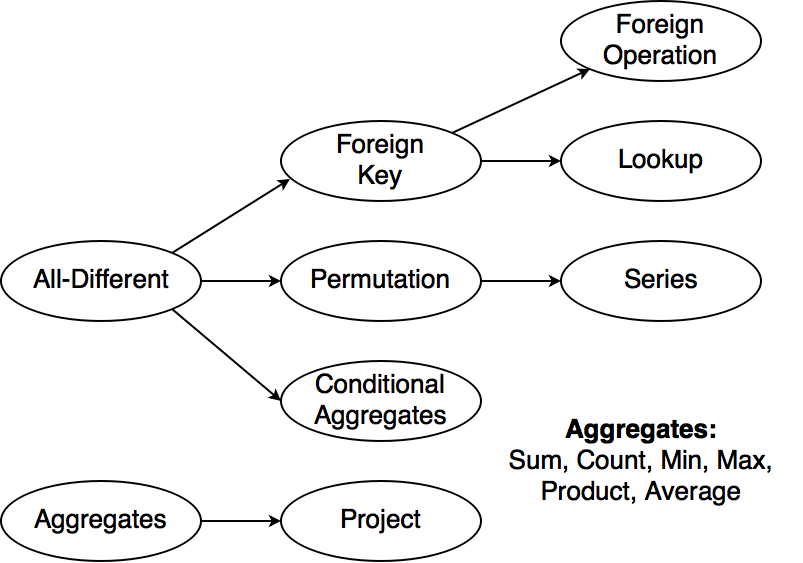
\includegraphics[width=0.20\textwidth]{figures/constraint_dependency.png}
  \caption{Constraint Learning Order. The solid arrows indicate a specificity order, i.e., \textit{permutation} $\rightarrow$ \textit{series} means that the series constraint is more specific than permutation. The dashed arrows indicate an inverse construction order, \textit{project} $\dashrightarrow$ \textit{aggregates} means the project constraint is more specific than aggregates. \sergey{Samuel,  can you give an explanation why we keep both arrow and how it is internally motivated?}}
  \label{fig:learning_order}
\end{figure}


\newcommand{\numeric}{\format{numeric}}
\newcommand{\textual}{\format{textual}}
\newcommand{\integer}{\format{integer}}
\newcommand{\length}{\format{length}}
\newcommand{\nat}{\mathcal{N}}

\sergey{Table should take into account our new notation and balance between formality and intuition, heh}
\begin{table*}
  \centering
  \begin{tabularx}{\textwidth}{XXX}
    \textbf{\CName} & \textbf{\CSignature} & \textbf{\CFunction}\\
    \ecalldiff{V_x} & X is integer or textual & All elements in X are different \\
    %X = Y & & \\
    \ecfkey{V_{fk}}{V_{pk}} & FK and PK have the same type; they originate from different tables and PK is all-different & all values in FK exist in PK \\
    % TODO check out
    \eclookupprod{V_r}{V_1}{V_{fk}}{V_{pk}}{V_{val}} & & \\
    \eclookup{V_r}{V_{fk}}{V_{pk}}{V_{val}} & & \\
    \eclookupfuzzy{V_r}{V_{fk}}{V_{pk}}{V_{val}} & & \\
    \ecperm{V_x} & & \\
    \ecprod{V_r}{V_1}{V_2} & & \\
    \ecproj{V_r}{G_x} & & \\
    \ecrank{V_r}{V_1} & Y and X have the same length & Y is the rank of X (including ties)\\
    \ectotal{V_r}{V_{pos}}{V_{neg}} & A, P and N have the same length and their length is at least 2 & *\\
    \ecseries{V_1} & & \\
    \ecsumc{V_r}{G_1} & & Y is the result of summing each column in X \\
    \ecsumr{V_r}{G_1} & & Y is the result of summing each row in X \\
    \ecsumif{V_r}{V_{fk}}{V_{pk}}{V_{val}} & & \\
    \ecsumprod{V_r}{V_1}{V_2} & & \\

\samuel{Motivate why product, not sum (=diff) you only need one, hardcoded preference for display}

  \end{tabularx}
  \caption{Spreadsheet Constraints \sergey{Here a detailed explanation on what is going on, what is essential, what is not? etc should be self-explanatory}}
  \label{table:constraints}
\end{table*}

% \subsection{Workflow}
% \begin{algorithm}[thb]
%   \begin{algorithmic}
%     \footnotesize
%     \State \textbf{Input:} $D$ -- dataset, \constraints -- constraints, \dependencies -- dependencies \\(optional: tables $T$, groups $G$)
%     \State \textbf{Output:} $S$ -- learned constraints with their satisfaction assignment
%     \If{$T$ is \textbf{not} provided}
%       \State $T \gets \extracttables(D)$
%     \EndIf
%     \If{$G$ is \textbf{not} provided}
%       \State $G \gets \extractgroups(D, T)$
%     \EndIf
%     \State $S \gets \learnconstraints(G,\constraints,\dependencies)$
%     \State \Return $S$
% \end{algorithmic}
% \caption{Workflow}
% \label{algo:workflow}
% \end{algorithm}

% \textbf{Approach}
% \begin{itemize}
%   \item Notation
%   \item Algorithm (select constraints, find assignments, find solutions)
% \end{itemize}

% \samuel{Move next to subgroup satisfaction search}
% \section{Declarative modeling}
% \sergey{We need to fit ASP, Minizinc and all that here, I mean it is supposed to be an important point after all}

\section{Evaluation}
In this section we experimentally validate our approach.
We studied various questions, most notably with what accuracy our algorithm can find essential constraints.

The implementation is illustrated using a case study on the spreadsheet corresponding with the previously introduced example (figure~\ref{fig:main_example}).
In order to quantify the results and generalize our findings we also evaluate our algorithm on a benchmark of 30 (\samuel{check number}) spreadsheets that we assembled from various sources.

In this section we focus on \textit{functional} constraints that could be used in spreadsheets, ignoring constraints such as all-different or foreign-key.

\subsection{Case study}
Let us illustrate our implementation using the example presented in Figure~\ref{fig:main_example}.
This example combines several smaller examples that were used in an exercise session to teach Excel into one spreadsheet.
Figure~\ref{fig:sol_example} shows the constraints that we expect to find.

\begin{figure}
  {\small
    \begin{align*}
      & SERIES(\range{T_{1}}{\rangeall}{1}) \\
%
      & \ecrank{\range{T_{1}}{\rangeall}{8}}{\range{T_{1}}{\rangeall}{7}} \\
%
      & \ecsumc{\range{T_{2}}{1}{\rangeall}}{\range{T_{1}}{\rangeall}{\rangeto{3}{7}}} \\
%
      & \ecsumc{\range{T_{6}}{\rangeall}{2}}{\range{T_{1}}{\rangeall}{\rangeto{3}{6}}} \\
%
      & \ecsumr{\range{T_{1}}{\rangeall}{7}}{\range{T_{1}}{\rangeall}{\rangeto{3}{6}}} \\
%
      & \ecaggc{AVERAGE}{\range{T_{2}}{2}{\rangeall}}{\range{T_{1}}{\rangeall}{\rangeto{3}{7}}} \\
%
      & \ecaggc{MAX}{\range{T_{2}}{3}{\rangeall}}{\range{T_{1}}{\rangeall}{\rangeto{3}{7}}} \\
%
      & \ecaggc{MIN}{\range{T_{2}}{4}{\rangeall}}{\range{T_{1}}{\rangeall}{\rangeto{3}{7}}} \\
%
      & \ecaggif{SUM}{\range{T_{1}}{\rangeall}{10}}{\range{T_{5}}{\rangeall}{1}}{\range{T_{1}}{\rangeall}{2}}{\range{T_{5}}{\rangeall}{2}} \\
%
      & \ecaggif{MAX}{\range{T_{1}}{\rangeall}{11}}{\range{T_{5}}{\rangeall}{1}}{\range{T_{1}}{\rangeall}{2}}{\range{T_{5}}{\rangeall}{2}} \\
%
      & \eclookup{\range{T_{4}}{\rangeall}{3}}{\range{T_{4}}{\rangeall}{2}}{\range{T_{1}}{\rangeall}{1}}{\range{T_{1}}{\rangeall}{2}} \\
%
      & \range{T_{6}}{\rangeall}{4} = PREV(\range{T_{6}}{\rangeall}{4}) + \range{T_{6}}{\rangeall}{2} - \range{T_{6}}{\rangeall}{3}
    \end{align*}
  }
  \caption{Expected constraints in the case study \sergey{in Figure \ref{fig:main_example}; some more explanation needed, not self explanatory}}
  \label{fig:sol_example}
\end{figure}
\sergey{Samuel, hint, don't put label before caption, it can't resolve it sometimes}

\subsubsection{Results}
\sergey{Samuel, you should just say at the beginning that all experiments has been run on macbook la-la system and that's it, I guess, I don't think we need to mention it multiple times}
Our current implementation takes a few seconds\footnote{3 seconds on our Macbook Pro} to find 18 constraints, including all of the 12 solutions described in Figure~\ref{fig:sol_example}.
Of the 6 remaining (redundant) constraints, 5 are $\mathit{RANK}$ constraints that are true by accident, such as: \begin{align*}
  & \ecrank{\range{T_1}{\rangeall}{1}}{\range{T_1}{\rangeall}{5}} \\
  & \ecrank{\range{T_1}{\rangeall}{8}}{\range{T_1}{\rangeall}{4}}
\end{align*}
The other redundant constraint is an additional $\mathit{LOOKUP}$ that holds because the vectors in \range{T_2}{\rangeall}{\rangeto{2}{3}} can both be used to look each other up in \range{T_1}{\rangeall}{\rangeto{1}{2}} and we considered only one of them to be essential (lookup using the ID).

For this example our primary goal of finding all constraints is achieved.
The implementation also returns a number of redundant constraints ($33.33\%$ of the total).
This ratio is, as we will show, rather high compared to other spreadsheets.
However, this example contains many short vectors which increases the chance for constraints to be true by accident.

\subsection{Benchmark}
There are three main categories of spreadsheets in the benchmark: spreadsheets from an exercise session teaching Excel at an affiliated University, spreadsheets from tutorials online and publicly available spreadsheets such as crime statistics or financial reports that demonstrate more real world usage\footnote{\samuel{link to links.txt}}.
The case study is also included.

All spreadsheets have been converted to CSV with no manual intervention unless noted.
Definitions of tables where added manually, providing a way to compare results and overcoming shortcomings in the table detection algorithm (in some harder cases groups where also provided manually).

For every spreadsheet a ground-truth has been provided manually, specifying the essential (or original) constraints that are expected to be discovered.
We consider three types of constraints:
\begin{description}
  \item[Expected] Constraint that have been implemented and are expected to be found
  \item[Essential] Constraint that have or have not been implemented but could be found using our algorithm
  \item[Non-trivial] Constraints currently outside of the scope of this system (e.g. generic nested mathematical or logical formulas or n-ary constraints)
\end{description}

\subsubsection*{Q1. How accurate is the approach?}
\sergey{that's confusing, it can do 100\% but then all of a sudden 96\%, short explanation needed}
Fortunately, our system is currently able to find $100\%$ of the expected constraints (90) on the benchmark suite.
There are only three essential constraints that have not been implemented yet, therefore our system currently identifies $96.77\%$ of the constraints that we hope to discover.

\subsubsection*{Q2. How many redundant constraints are discovered?}
Our primary focus was accuracy, therefore we sometimes traded off less redundancy for more accuracy.
The motivation is that solutions can still be pruned using entailment or heuristics afterwards.
The constraints we considered to be redundant are either duplications (results that can be calculated in different ways, one of which seems superior) or constraints that hold by accident.
Duplications should be detected in a post-processing step while accidental constraints should primarily be removed by adding data.

Across all spreadsheets our implementation finds 121 constraints, 28 ($23.14\%$) of which are redundant.
However, the average redundancy per spreadsheet is only $8.33\%$.
Examining the redundant constraints reveals that many (12) of them are duplications occurring in a single spreadsheet.
Many of the remaining constraints are duplications stemming from the overlapping role of difference and sum.
Accidental constraints are limited to the 5 rank constraints that were discussed in the case study.

\subsubsection*{Q3. How fast is the algorithm?}
Concerning the speed of the algorithm we also prioritized accuracy when a trade-off had to be made.
For the 32 spreadsheets in the benchmark our implementation ran in $17.86s \pm 0.87s$\footnote{Macbook Pro, Intel Core i7 2.3 GHz, 16GB RAM}.
The execution times vary widely though between spreadsheets, only four spreadsheets taking more than $0.2s$.
Most of the execution time in these cases goes towards searching either aggregate constraints or conditional aggregates.
The search for aggregates will be slow on spreadsheets containing larger groups of numeric data.
For conditional aggregates the number of candidate primary keys (all-different) and numeric vectors determines the running time (e.g. the case study example).

\paragraph{Dependencies}
In order for the algorithm to run efficiently it is crucial to use dependencies and find constraint incrementally whenever possible.
This avoids some of the explosion of combinations for constraints that have variables.
For example, using foreign keys as a base constraint to find conditional aggregates reduces the running time for the case study from about 3 seconds to under 1 second.
Unfortunately, this assumption is sometimes too strong, when users are interested in aggregates for only some of the keys present.

\subsection{Insights}
\sergey{We should explain Figure \ref{fig:fbi}, e.g. if we aggregate by the crime now, the missing value would not get into statistics, which seems faulty, since we can directly compute it.}

\begin{figure*}[thb]
  \begin{center}
    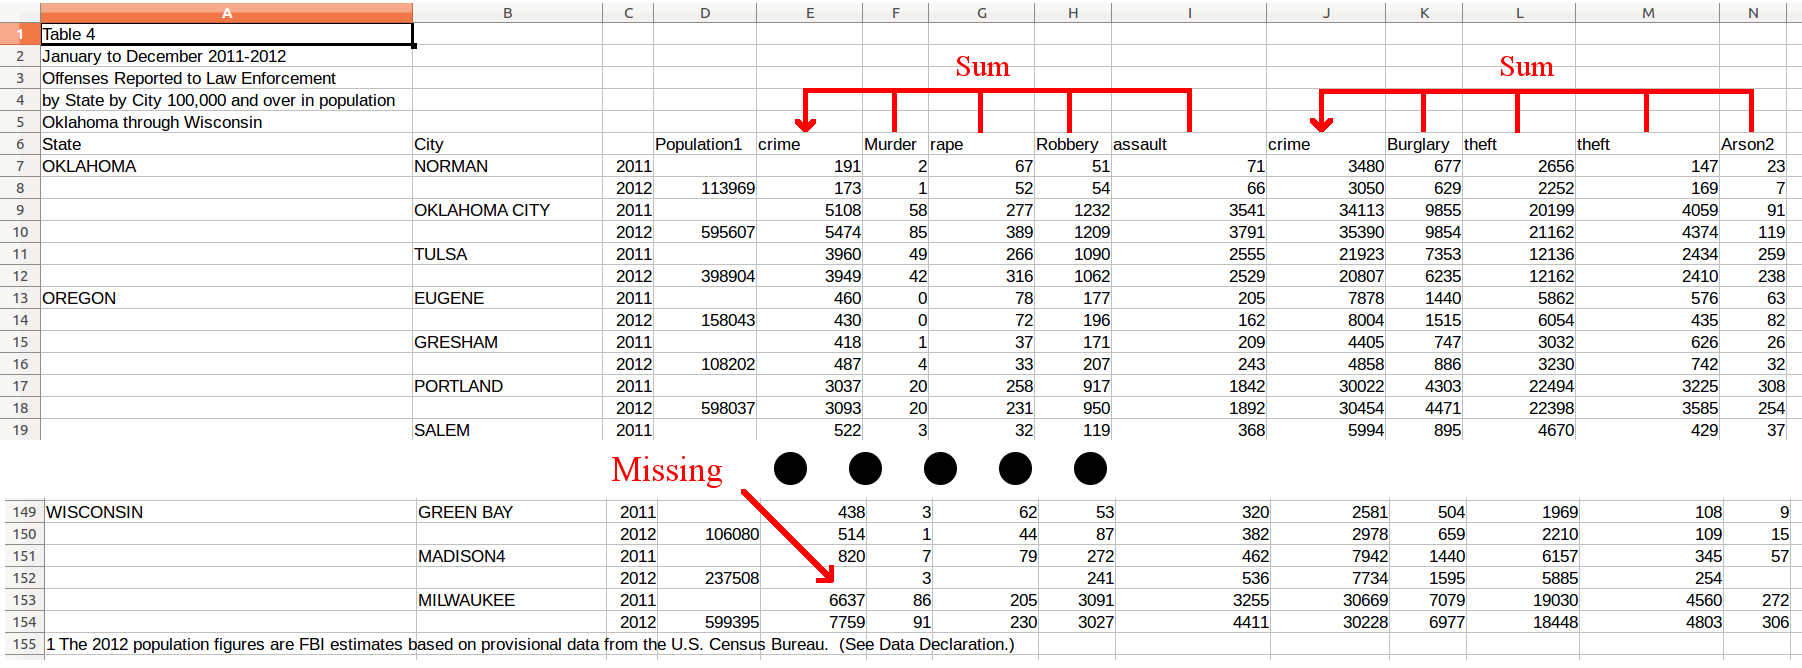
\includegraphics[width=0.85\textwidth]{figures/fbi_figure_highlighted.png}
  \end{center}
  \caption{Real world tabular constraint reconstruction: FBI crime statistics}
  \label{fig:fbi}
\end{figure*}


\sergey{I think there should be three things: key example evaluated, benchmark of 30 spreadsheets and maybe the FBI example, how we can detect interesting dependencies and correct potential mistakes}


{\bfseries
  Experimental questions
}

\begin{itemize}
  \item  How accurate are we? (Accuracy / recall)
  \item  How fast are we and which factors affect the runtime (how)?
  \item  How general is our approach, what limitations are there?
\end{itemize}


\section{Related Work}
\sergey{key bullet points for Luc and possibly Samuel and me to make related work section}

\sergey{ECAI reference style file ignores their guideline and their guideline ignores what is written in the guidelines!}
flashfill, flashextract, flashmeta \cite{flashfill,flashextract,flashmeta}
\begin{itemize}
  \item their supervised vs our unsupervised approach
  \item they look for a single ``smallest'' solution, we enumerate them all
  \item they are looking for a function, we solve constraint satisfaction problems
  \item we do not assume classic row based data layout, we work in the tabular setting
\end{itemize}

sketch \cite{sketch}
\begin{itemize}
  \item look for a constant that would fill in the gap in a program
  \item tailored for programming languages
  \item similar to model checking
  \item looks for a single solution
  \item similar to constraint satisfaction and sat, where one is interested in a single assignment that works for any potential input
\end{itemize}

tabular \cite{tabular}
\begin{itemize}
  \item language based on the excel tables that specify probabilistic models
  \item a system for probabilistic inference and similarity mostly in the usage of excel
  \item probabilistic constraint satisfaction (?) and graphical models
  \item single solution again
\end{itemize}

modelseeker \cite{modelseeker} \sergey{Samuel, Luc, probably you would need elaborate here more in details}

\begin{itemize}
  \item not designed for excel-like data representation (type consistency, groups, etc)
  \item not designed for excel-like constraints (lookups, conditional ifs, etc)
  \item does not support user extensions (?)
\end{itemize}

claudien \cite{claudien} \sergey{Samuel, Luc, you would need to help with this one}

\section{Discussion and Conclusions}
\sergey{link to the github with implementations and the dataset}


\sergey{Future version, extensions, declarative stuff, bla-bla here}

\bibliographystyle{ecai}
\bibliography{references}
\end{document}
%%%%%%%%%%%%%%%%%%%%%%%%%%%%%%%%%%%%%%%%%%%%%%%%%%%%%%%%%%%%%%%%%%%%%%
